\documentclass[11pt]{article}

\usepackage[right=0.5in,left=0.5in, landscape]{geometry}
\usepackage{url}
\usepackage{fancyhdr}
\pagestyle{fancy}
\usepackage{amsmath}
\usepackage{amssymb}
\usepackage{color}
\usepackage{graphicx}
\usepackage{listings}
\usepackage{sectsty}
\sectionfont{\large}

\lhead{Intro to Parallel Comp PA2}
\chead{Melvyn Ian Drag}
\rhead{\today}
\setlength{\parskip}{0pt} 
\setlength{\parindent}{0pt}

\allowdisplaybreaks

\begin{document}
I used the template provided by the professor. I am including here the functions I modified (I also added a couple of lines near the top to define block size, chunk size, and the number of threads), and a bit of information about the performance I achieved. I am also including a printout of the results of the codes and the GFLOPS attained. The clear winner is to assign chunks of rows to different cores.
But first, here is an image of how I parallelized.
\begin{center}
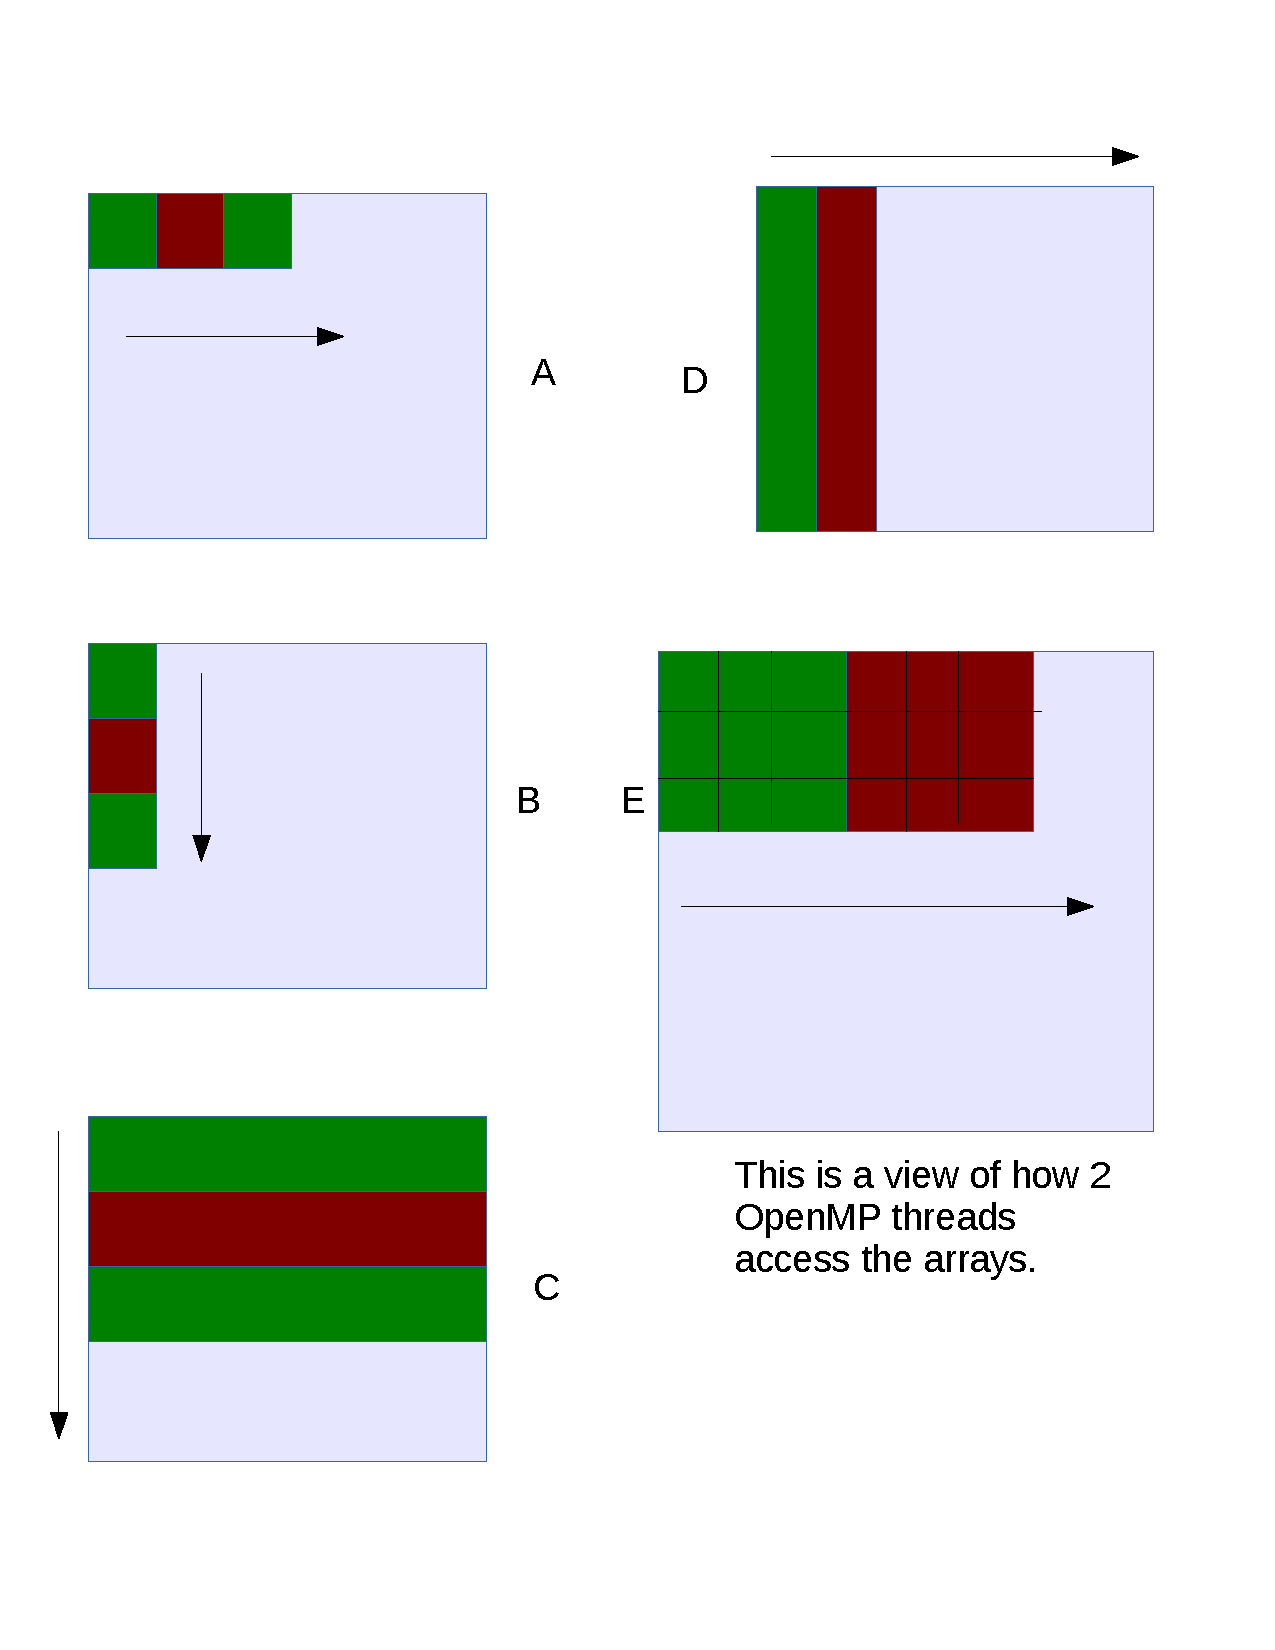
\includegraphics[scale=0.45]{/home/melvyn/Documents/IntroToParallel/PA2/done/openmp.pdf}
\end{center}
\section{Sequential Code Performance}
 \begin{lstlisting}
--------------------------------------------------------------
Compiling Programming Assignment 2 Serial Version
--------------------------------------------------------------
 
 
GCC: Serial
 
Iter = 0 Resid Norm = 905946.143408
Iter = 10 Resid Norm = 96894.410256
Iter = 20 Resid Norm = 10380.708983
Iter = 30 Resid Norm = 1112.668792
Iter = 40 Resid Norm = 119.293944
Iter = 50 Resid Norm = 12.792188
Iter = 60 Resid Norm = 1.371906
Iter = 70 Resid Norm = 0.147145
Iter = 80 Resid Norm = 0.015783
Iter = 90 Resid Norm = 0.001693
Iter = 100 Resid Norm = 0.000182
Iter = 110 Resid Norm = 0.000019
Iter = 120 Resid Norm = 0.000002
Solution converged in 124 iterations
Final residual norm = 0.000001
Solution at center and four corners of interior N/2 by N/2 grid : 
xnew[256][256]=512.000000
xnew[256][769]=1025.000000
xnew[512][512]=1024.000000
xnew[769][256]=1025.000000
xnew[769][769]=1538.000000
Sequential Jacobi: Matrix Size = 1024; 1.4 GFLOPS; Time = 1.213 sec; 
\end{lstlisting}

\section{Parallel Performance of Methods a-e on 2 Cores}

\begin{lstlisting}
 
--------------------------------------------------------------
Compiling Programming Assignment 2 With 2 Processors
--------------------------------------------------------------
 
 
GCC: Run a
 
Iter = 0 Resid Norm = 905946.143408
Iter = 10 Resid Norm = 96894.410256
Iter = 20 Resid Norm = 10380.708983
Iter = 30 Resid Norm = 1112.668792
Iter = 40 Resid Norm = 119.293944
Iter = 50 Resid Norm = 12.792188
Iter = 60 Resid Norm = 1.371906
Iter = 70 Resid Norm = 0.147145
Iter = 80 Resid Norm = 0.015783
Iter = 90 Resid Norm = 0.001693
Iter = 100 Resid Norm = 0.000182
Iter = 110 Resid Norm = 0.000019
Iter = 120 Resid Norm = 0.000002
Solution converged in 124 iterations
Final residual norm = 0.000001
Solution at center and four corners of interior N/2 by N/2 grid : 
xnew[256][256]=512.000000
xnew[256][769]=1025.000000
xnew[512][512]=1024.000000
xnew[769][256]=1025.000000
xnew[769][769]=1538.000000
Sequential Jacobi: Matrix Size = 1024; 0.2 GFLOPS; Time = 9.414 sec; 
 
GCC: Run b
 
Iter = 0 Resid Norm = 905946.143408
Iter = 10 Resid Norm = 96894.410256
Iter = 20 Resid Norm = 10380.708983
Iter = 30 Resid Norm = 1112.668792
Iter = 40 Resid Norm = 119.293944
Iter = 50 Resid Norm = 12.792188
Iter = 60 Resid Norm = 1.371906
Iter = 70 Resid Norm = 0.147145
Iter = 80 Resid Norm = 0.015783
Iter = 90 Resid Norm = 0.001693
Iter = 100 Resid Norm = 0.000182
Iter = 110 Resid Norm = 0.000019
Iter = 120 Resid Norm = 0.000002
Solution converged in 124 iterations
Final residual norm = 0.000001
Solution at center and four corners of interior N/2 by N/2 grid : 
xnew[256][256]=512.000000
xnew[256][769]=1025.000000
xnew[512][512]=1024.000000
xnew[769][256]=1025.000000
xnew[769][769]=1538.000000
Sequential Jacobi: Matrix Size = 1024; 0.1 GFLOPS; Time = 14.920 sec; 
 
GCC: Run c
 
Iter = 0 Resid Norm = 12277426.934435
Iter = 10 Resid Norm = 1314641.172881
Iter = 20 Resid Norm = 140935.129160
Iter = 30 Resid Norm = 15113.972965
Iter = 40 Resid Norm = 1621.128747
Iter = 50 Resid Norm = 173.903416
Iter = 60 Resid Norm = 18.656744
Iter = 70 Resid Norm = 2.005477
Iter = 80 Resid Norm = 0.214769
Iter = 90 Resid Norm = 0.023045
Iter = 100 Resid Norm = 0.002473
Iter = 110 Resid Norm = 0.000265
Iter = 120 Resid Norm = 0.000028
Iter = 130 Resid Norm = 0.000003
Solution converged in 135 iterations
Final residual norm = 0.000001
Solution at center and four corners of interior N/2 by N/2 grid : 
xnew[256][256]=512.000000
xnew[256][769]=1025.000000
xnew[512][512]=1024.000000
xnew[769][256]=1025.000000
xnew[769][769]=1538.000000
Sequential Jacobi: Matrix Size = 1024; 2.5 GFLOPS; Time = 0.730 sec; 
 
GCC: Run d
 
Iter = 0 Resid Norm = 2260838.587495
Iter = 10 Resid Norm = 242038.951349
Iter = 20 Resid Norm = 25944.948887
Iter = 30 Resid Norm = 2782.141135
Iter = 40 Resid Norm = 298.447683
Iter = 50 Resid Norm = 32.008025
Iter = 60 Resid Norm = 3.439798
Iter = 70 Resid Norm = 0.368388
Iter = 80 Resid Norm = 0.039525
Iter = 90 Resid Norm = 0.004242
Iter = 100 Resid Norm = 0.000455
Iter = 110 Resid Norm = 0.000049
Iter = 120 Resid Norm = 0.000005
Solution converged in 128 iterations
Final residual norm = 0.000001
Solution at center and four corners of interior N/2 by N/2 grid : 
xnew[256][256]=512.000000
xnew[256][769]=1025.000000
xnew[512][512]=1024.000000
xnew[769][256]=1025.000000
xnew[769][769]=1538.000000
Sequential Jacobi: Matrix Size = 1024; 1.1 GFLOPS; Time = 1.652 sec; 
 
GCC: Run e
 
Iter = 0 Resid Norm = 1353816.547936
Iter = 10 Resid Norm = 144900.772545
Iter = 20 Resid Norm = 15530.254727
Iter = 30 Resid Norm = 1665.168657
Iter = 40 Resid Norm = 178.579059
Iter = 50 Resid Norm = 19.154161
Iter = 60 Resid Norm = 2.054656
Iter = 70 Resid Norm = 0.220418
Iter = 80 Resid Norm = 0.023647
Iter = 90 Resid Norm = 0.002537
Iter = 100 Resid Norm = 0.000272
Iter = 110 Resid Norm = 0.000029
Iter = 120 Resid Norm = 0.000003
Solution converged in 126 iterations
Final residual norm = 0.000001
Solution at center and four corners of interior N/2 by N/2 grid : 
xnew[256][256]=512.000000
xnew[256][769]=1025.000000
xnew[512][512]=1024.000000
xnew[769][256]=1025.000000
xnew[769][769]=1538.000000
Sequential Jacobi: Matrix Size = 1024; 1.7 GFLOPS; Time = 1.005 sec; 

-----------------------
Resources requested:
mem=48gb
nodes=1:ppn=12
-----------------------
Resources used:
cput=00:01:06
walltime=00:00:36
mem=0.034 GB
vmem=0.153 GB
-----------------------
Resource units charged (estimate):
0.012 RUs
-----------------------
\end{lstlisting}
\section{Parallel Performance of Methods a-e on 4 Cores}
\begin{lstlisting}
 
--------------------------------------------------------------
Compiling Programming Assignment 2 With 4 Cores
--------------------------------------------------------------
 
 
GCC: Run a
 
Iter = 0 Resid Norm = 905946.143408
Iter = 10 Resid Norm = 96894.410256
Iter = 20 Resid Norm = 10380.708983
Iter = 30 Resid Norm = 1112.668792
Iter = 40 Resid Norm = 119.293944
Iter = 50 Resid Norm = 12.792188
Iter = 60 Resid Norm = 1.371906
Iter = 70 Resid Norm = 0.147145
Iter = 80 Resid Norm = 0.015783
Iter = 90 Resid Norm = 0.001693
Iter = 100 Resid Norm = 0.000182
Iter = 110 Resid Norm = 0.000019
Iter = 120 Resid Norm = 0.000002
Solution converged in 124 iterations
Final residual norm = 0.000001
Solution at center and four corners of interior N/2 by N/2 grid : 
xnew[256][256]=512.000000
xnew[256][769]=1025.000000
xnew[512][512]=1024.000000
xnew[769][256]=1025.000000
xnew[769][769]=1538.000000
Sequential Jacobi: Matrix Size = 1024; 0.2 GFLOPS; Time = 10.663 sec; 
 
GCC: Run b
 
Iter = 0 Resid Norm = 905946.143408
Iter = 10 Resid Norm = 96894.410256
Iter = 20 Resid Norm = 10380.708983
Iter = 30 Resid Norm = 1112.668792
Iter = 40 Resid Norm = 119.293944
Iter = 50 Resid Norm = 12.792188
Iter = 60 Resid Norm = 1.371906
Iter = 70 Resid Norm = 0.147145
Iter = 80 Resid Norm = 0.015783
Iter = 90 Resid Norm = 0.001693
Iter = 100 Resid Norm = 0.000182
Iter = 110 Resid Norm = 0.000019
Iter = 120 Resid Norm = 0.000002
Solution converged in 124 iterations
Final residual norm = 0.000001
Solution at center and four corners of interior N/2 by N/2 grid : 
xnew[256][256]=512.000000
xnew[256][769]=1025.000000
xnew[512][512]=1024.000000
xnew[769][256]=1025.000000
xnew[769][769]=1538.000000
Sequential Jacobi: Matrix Size = 1024; 0.2 GFLOPS; Time = 11.183 sec; 
 
GCC: Run c
 
Iter = 0 Resid Norm = 8789920.587727
Iter = 10 Resid Norm = 934195.049495
Iter = 20 Resid Norm = 99982.167666
Iter = 30 Resid Norm = 10784.555929
Iter = 40 Resid Norm = 1150.734832
Iter = 50 Resid Norm = 124.090146
Iter = 60 Resid Norm = 13.234581
Iter = 70 Resid Norm = 1.432201
Iter = 80 Resid Norm = 0.153191
Iter = 90 Resid Norm = 0.016441
Iter = 100 Resid Norm = 0.001760
Iter = 110 Resid Norm = 0.000189
Iter = 120 Resid Norm = 0.000020
Iter = 130 Resid Norm = 0.000002
Solution converged in 134 iterations
Final residual norm = 0.000001
Solution at center and four corners of interior N/2 by N/2 grid : 
xnew[256][256]=512.000000
xnew[256][769]=1025.000000
xnew[512][512]=1024.000000
xnew[769][256]=1025.000000
xnew[769][769]=1538.000000
Sequential Jacobi: Matrix Size = 1024; 3.3 GFLOPS; Time = 0.558 sec; 
 
GCC: Run d
 
Iter = 0 Resid Norm = 1664850.217475
Iter = 10 Resid Norm = 178202.877494
Iter = 20 Resid Norm = 19100.241448
Iter = 30 Resid Norm = 2048.005911
Iter = 40 Resid Norm = 219.641441
Iter = 50 Resid Norm = 23.558977
Iter = 60 Resid Norm = 2.527208
Iter = 70 Resid Norm = 0.271118
Iter = 80 Resid Norm = 0.029087
Iter = 90 Resid Norm = 0.003121
Iter = 100 Resid Norm = 0.000335
Iter = 110 Resid Norm = 0.000036
Iter = 120 Resid Norm = 0.000004
Solution converged in 127 iterations
Final residual norm = 0.000001
Solution at center and four corners of interior N/2 by N/2 grid : 
xnew[256][256]=512.000000
xnew[256][769]=1025.000000
xnew[512][512]=1024.000000
xnew[769][256]=1025.000000
xnew[769][769]=1538.000000
Sequential Jacobi: Matrix Size = 1024; 2.0 GFLOPS; Time = 0.876 sec; 
 
GCC: Run e
 
Iter = 0 Resid Norm = 1353816.547936
Iter = 10 Resid Norm = 144900.772545
Iter = 20 Resid Norm = 15530.254727
Iter = 30 Resid Norm = 1665.168657
Iter = 40 Resid Norm = 178.579059
Iter = 50 Resid Norm = 19.154161
Iter = 60 Resid Norm = 2.054656
Iter = 70 Resid Norm = 0.220418
Iter = 80 Resid Norm = 0.023647
Iter = 90 Resid Norm = 0.002537
Iter = 100 Resid Norm = 0.000272
Iter = 110 Resid Norm = 0.000029
Iter = 120 Resid Norm = 0.000003
Solution converged in 126 iterations
Final residual norm = 0.000001
Solution at center and four corners of interior N/2 by N/2 grid : 
xnew[256][256]=512.000000
xnew[256][769]=1025.000000
xnew[512][512]=1024.000000
xnew[769][256]=1025.000000
xnew[769][769]=1538.000000
Sequential Jacobi: Matrix Size = 1024; 1.7 GFLOPS; Time = 1.008 sec; 

-----------------------
Resources requested:
mem=48gb
nodes=1:ppn=12
-----------------------
Resources used:
cput=00:01:46
walltime=00:00:29
mem=0.034 GB
vmem=0.157 GB
-----------------------
Resource units charged (estimate):
0.009 RUs
-----------------------
\end{lstlisting}
\section{Parallel Performance of Methods a-e on 8 Cores}
\begin{lstlisting}
 
--------------------------------------------------------------
Compiling Programming Assignment 2 With 8 Cores
--------------------------------------------------------------
 
 
GCC: Run a
 
Iter = 0 Resid Norm = 905946.143408
Iter = 10 Resid Norm = 96894.410256
Iter = 20 Resid Norm = 10380.708983
Iter = 30 Resid Norm = 1112.668792
Iter = 40 Resid Norm = 119.293944
Iter = 50 Resid Norm = 12.792188
Iter = 60 Resid Norm = 1.371906
Iter = 70 Resid Norm = 0.147145
Iter = 80 Resid Norm = 0.015783
Iter = 90 Resid Norm = 0.001693
Iter = 100 Resid Norm = 0.000182
Iter = 110 Resid Norm = 0.000019
Iter = 120 Resid Norm = 0.000002
Solution converged in 124 iterations
Final residual norm = 0.000001
Solution at center and four corners of interior N/2 by N/2 grid : 
xnew[256][256]=512.000000
xnew[256][769]=1025.000000
xnew[512][512]=1024.000000
xnew[769][256]=1025.000000
xnew[769][769]=1538.000000
Sequential Jacobi: Matrix Size = 1024; 0.1 GFLOPS; Time = 15.593 sec; 
 
GCC: Run b
 
Iter = 0 Resid Norm = 905946.143408
Iter = 10 Resid Norm = 96894.410256
Iter = 20 Resid Norm = 10380.708983
Iter = 30 Resid Norm = 1112.668792
Iter = 40 Resid Norm = 119.293944
Iter = 50 Resid Norm = 12.792188
Iter = 60 Resid Norm = 1.371906
Iter = 70 Resid Norm = 0.147145
Iter = 80 Resid Norm = 0.015783
Iter = 90 Resid Norm = 0.001693
Iter = 100 Resid Norm = 0.000182
Iter = 110 Resid Norm = 0.000019
Iter = 120 Resid Norm = 0.000002
Solution converged in 124 iterations
Final residual norm = 0.000001
Solution at center and four corners of interior N/2 by N/2 grid : 
xnew[256][256]=512.000000
xnew[256][769]=1025.000000
xnew[512][512]=1024.000000
xnew[769][256]=1025.000000
xnew[769][769]=1538.000000
Sequential Jacobi: Matrix Size = 1024; 0.2 GFLOPS; Time = 10.633 sec; 
 
GCC: Run c
 
Iter = 0 Resid Norm = 6384960.495819
Iter = 10 Resid Norm = 684652.320061
Iter = 20 Resid Norm = 75639.266845
Iter = 30 Resid Norm = 7869.630370
Iter = 40 Resid Norm = 851.077427
Iter = 50 Resid Norm = 90.669047
Iter = 60 Resid Norm = 9.778769
Iter = 70 Resid Norm = 1.046775
Iter = 80 Resid Norm = 0.111001
Iter = 90 Resid Norm = 0.011961
Iter = 100 Resid Norm = 0.001311
Iter = 110 Resid Norm = 0.000141
Iter = 120 Resid Norm = 0.000015
Iter = 130 Resid Norm = 0.000002
Solution converged in 133 iterations
Final residual norm = 0.000001
Solution at center and four corners of interior N/2 by N/2 grid : 
xnew[256][256]=512.000000
xnew[256][769]=1025.000000
xnew[512][512]=1024.000000
xnew[769][256]=1025.000000
xnew[769][769]=1538.000000
Sequential Jacobi: Matrix Size = 1024; 3.6 GFLOPS; Time = 0.507 sec; 
 
GCC: Run d
 
Iter = 0 Resid Norm = 1281676.473898
Iter = 10 Resid Norm = 135901.865959
Iter = 20 Resid Norm = 14689.446578
Iter = 30 Resid Norm = 1561.433103
Iter = 40 Resid Norm = 172.499279
Iter = 50 Resid Norm = 17.958294
Iter = 60 Resid Norm = 1.982370
Iter = 70 Resid Norm = 0.214274
Iter = 80 Resid Norm = 0.022167
Iter = 90 Resid Norm = 0.002456
Iter = 100 Resid Norm = 0.000258
Iter = 110 Resid Norm = 0.000028
Iter = 120 Resid Norm = 0.000003
Solution converged in 125 iterations
Final residual norm = 0.000001
Solution at center and four corners of interior N/2 by N/2 grid : 
xnew[256][256]=512.000000
xnew[256][769]=1025.000000
xnew[512][512]=1024.000000
xnew[769][256]=1025.000000
xnew[769][769]=1538.000000
Sequential Jacobi: Matrix Size = 1024; 2.6 GFLOPS; Time = 0.673 sec; 
 
GCC: Run e
 
Iter = 0 Resid Norm = 1353816.547936
Iter = 10 Resid Norm = 144900.772545
Iter = 20 Resid Norm = 15530.254727
Iter = 30 Resid Norm = 1665.168657
Iter = 40 Resid Norm = 178.579059
Iter = 50 Resid Norm = 19.154161
Iter = 60 Resid Norm = 2.054656
Iter = 70 Resid Norm = 0.220418
Iter = 80 Resid Norm = 0.023647
Iter = 90 Resid Norm = 0.002537
Iter = 100 Resid Norm = 0.000272
Iter = 110 Resid Norm = 0.000029
Iter = 120 Resid Norm = 0.000003
Solution converged in 126 iterations
Final residual norm = 0.000001
Solution at center and four corners of interior N/2 by N/2 grid : 
xnew[256][256]=512.000000
xnew[256][769]=1025.000000
xnew[512][512]=1024.000000
xnew[769][256]=1025.000000
xnew[769][769]=1538.000000
Sequential Jacobi: Matrix Size = 1024; 1.7 GFLOPS; Time = 1.029 sec; 

-----------------------
Resources requested:
mem=48gb
nodes=1:ppn=12
-----------------------
Resources used:
cput=00:03:53
walltime=00:00:31
mem=0.034 GB
vmem=0.165 GB
-----------------------
Resource units charged (estimate):
0.010 RUs
-----------------------
\end{lstlisting}
\section{Worksharing Across Rows}
\begin{lstlisting}

double rhocalc(double * A)
{
	//Parallelize this
	double tmp, temp;
	int i,j;
	tmp = 0.0;
	temp = 0.0;
	for(i=1;i<N+1;i++)
	{
		#pragma omp parallel for shared(A) num_threads(NUM_THREADS)\
			schedule(dynamic, CHUNK_SIZE)
		for(j=1;j<N+1;j++)
			#pragma omp atomic
			tmp+=A[i*(N+2)+j]*A[i*(N+2)+j];
			// This is a terrible solution
	}
	return(sqrt(tmp));
}

void update(double * xold,double * xnew,double * resid, double * b)
{
  //Parallelize this
  int i,j;
  for(i=1;i<N+1;i++)
	#pragma omp parallel for shared(xnew, xold) num_threads(NUM_THREADS)\
		schedule(dynamic, CHUNK_SIZE)
    for(j=1;j<N+1;j++){
      xnew[i*(N+2)+j]=b[i*(N+2)+j]-odiag*(xold[i*(N+2)+j-1]+xold[i*(N+2)+j+1]+\
	    xold[(i+1)*(N+2)+j]+xold[(i-1)*(N+2)+j]);
      xnew[i*(N+2)+j]*=recipdiag;
    }
  for(i=1;i<N+1;i++)
  	#pragma omp parallel for shared(xnew, resid) num_threads(NUM_THREADS)\
		schedule(dynamic, CHUNK_SIZE)
    for(j=1;j<N+1;j++)
    {
      resid[i*(N+2)+j]=b[i*(N+2)+j]-diag*xnew[i*(N+2)+j]-odiag*(xnew[i*(N+2)+j+1]+\
           xnew[i*(N+2)+j-1]+xnew[(i-1)*(N+2)+j]+xnew[(i+1)*(N+2)+j]);
    } 
} 
  
void copy(double * xold, double * xnew)
{
	//Parallelize this
	int i,j;
	for(i=1;i<N+1;i++)
		#pragma omp parallel for shared(xnew, xold) num_threads(NUM_THREADS)\
			schedule(dynamic, CHUNK_SIZE)
		for(j=1;j<N+1;j++)
			xold[i*(N+2)+j]=xnew[i*(N+2)+j];
}

\end{lstlisting}

\section{Work Sharing Across Columns}
\begin{lstlisting}

double rhocalc(double * A)
{
	//Parallelize this
	double tmp;	tmp = 0.0;
	int i,j;
	for(j=1;j<N+1;j++)
	{ 
		#pragma omp parallel for num_threads(NUM_THREADS) schedule(dynamic, CHUNK_SIZE)
		for(i=1;i<N+1;i++)
		{	
			#pragma omp atomic
			tmp+=A[i*(N+2)+j]*A[i*(N+2)+j];
		}
	}
	return(sqrt(tmp));
}

void update(double * xold,double * xnew,double * resid, double * b)
{
	//Parallelize this
	int i,j;
	for(j=1;j<N+1;j++)
		#pragma omp parallel for num_threads(NUM_THREADS) schedule(dynamic, CHUNK_SIZE)
		for(i=1;i<N+1;i++)
		{
			xnew[i*(N+2)+j]=b[i*(N+2)+j]-odiag*(xold[i*(N+2)+j-1]+xold[i*(N+2)+j+1]+\
				xold[(i+1)*(N+2)+j]+xold[(i-1)*(N+2)+j]);
			xnew[i*(N+2)+j]*=recipdiag;
		}
	for(j=1;j<N+1;j++)
		#pragma omp parallel for num_threads(NUM_THREADS) schedule(dynamic, CHUNK_SIZE)
		for(i=1;i<N+1;i++)
		{
			resid[i*(N+2)+j]=b[i*(N+2)+j]-diag*xnew[i*(N+2)+j]-odiag*(xnew[i*(N+2)+j+1]+\
				xnew[i*(N+2)+j-1]+xnew[(i-1)*(N+2)+j]+xnew[(i+1)*(N+2)+j]);
		} 
} 
  
void copy(double * xold, double * xnew)
{
	//Parallelize this
	int i,j;
	for(j=1;j<N+1;j++)
		#pragma omp parallel for num_threads(NUM_THREADS) schedule(dynamic, CHUNK_SIZE)
		for(i=1;i<N+1;i++)
			xold[i*(N+2)+j]=xnew[i*(N+2)+j];
}
\end{lstlisting}
\section{1D domain decomposition along rows of the matrices}
\begin{lstlisting}
double rhocalc(double * A)
{
	//Parallelize this
	double tmp, temp;
	int i,j;
	tmp = 0.0;
	temp = 0.0;
	#pragma omp parallel for private(j) firstprivate(temp)\
		schedule(dynamic, CHUNK_SIZE) num_threads(NUM_THREADS)
	for(i=1;i<N+1;i++)
	{
		for(j=1;j<N+1;j++)
			temp+=A[i*(N+2)+j]*A[i*(N+2)+j];
		#pragma omp atomic
		tmp += temp;
	}
	return(sqrt(tmp));
}

void update(double * xold,double * xnew,double * resid, double * b)
{
	//Parallelize this
	int i,j;
	#pragma omp parallel for schedule(dynamic, CHUNK_SIZE) num_threads(NUM_THREADS) \
		private(j) shared(xold, xnew)
	for(i=1;i<N+1;i++)
		for(j=1;j<N+1;j++)
		{
			// Although different threads will be accessing the same data elements,
			//  they will likely not do this at the same time. This is to say,even
			// though the accesses to xold overlap a bit due to the + 1 and -1 in 
			// the indexing (with respect to i), the overlap in accesses will likely
			// be at different times, so there will be no cache thrasing.
			xnew[i*(N+2)+j]=b[i*(N+2)+j]-odiag*(xold[i*(N+2)+j-1]+xold[i*(N+2)+j+1]+\
				xold[(i+1)*(N+2)+j]+xold[(i-1)*(N+2)+j]);
			xnew[i*(N+2)+j]*=recipdiag;
		}
	#pragma omp parallel for private(j) schedule(dynamic, CHUNK_SIZE) \
		num_threads(NUM_THREADS) shared (resid, xnew)
	for(i=1;i<N+1;i++)
		for(j=1;j<N+1;j++)
		{
			// Similarly to (above), there is some overlap in the data elements of xnew accessed
			// between threads, but these accesses will likely occur at different times, so there 
			// will be little cache thrashing.
			resid[i*(N+2)+j]=b[i*(N+2)+j]-diag*xnew[i*(N+2)+j]-odiag*(xnew[i*(N+2)+j+1]+\
				xnew[i*(N+2)+j-1]+xnew[(i-1)*(N+2)+j]+xnew[(i+1)*(N+2)+j]);
		} 
} 
  
void copy(double * xold, double * xnew)	
{
	//Parallelize this
	int i,j;
	#pragma omp parallel for private(j) schedule(dynamic, CHUNK_SIZE) \
		num_threads(NUM_THREADS) shared(xold, xnew)
	for(i=1;i<N+1;i++)
		for(j=1;j<N+1;j++)
			xold[i*(N+2)+j]=xnew[i*(N+2)+j];
}

\end{lstlisting}
\section{1D domain decomposition along columns of the matrices}
\begin{lstlisting}
double rhocalc(double * A)
{
	//Parallelize this
	double tmp, temp;
	int i,j, jt;
	tmp = 0.0; temp = 0.0;
	#pragma omp parallel for private(i,j) schedule(dynamic, CHUNK_SIZE) num_threads(NUM_THREADS) firstprivate(temp) 
	for(jt = 1; jt < N+1; jt+=BLOCK_SIZE)
	{
		for(i=1;i<N+1;i++)
			for(j=jt;j<jt+BLOCK_SIZE;j++)
				temp+=A[i*(N+2)+j]*A[i*(N+2)+j];
		#pragma omp atomic
		tmp += temp;
	}
	return(sqrt(tmp));
}


void update(double * xold,double * xnew,double * resid, double * b)
{
	//Parallelize this
	int i,j, jt;
	#pragma omp parallel for private(i,j) schedule(dynamic, CHUNK_SIZE)\
		num_threads(NUM_THREADS) shared(xnew, xold) 
	for(jt = 1; jt < N+1; jt+=BLOCK_SIZE)
		for(i=1;i<N+1;i++)
			for(j=jt;j<jt+BLOCK_SIZE;j++)
			{
				xnew[i*(N+2)+j]=b[i*(N+2)+j]-odiag*(xold[i*(N+2)+j-1]+xold[i*(N+2)+j+1]+\
					xold[(i+1)*(N+2)+j]+xold[(i-1)*(N+2)+j]);
				xnew[i*(N+2)+j]*=recipdiag;
			}
	#pragma omp parallel for private(i,j) schedule(dynamic, CHUNK_SIZE) \
		num_threads(NUM_THREADS) shared(resid, xnew)
	for(jt = 1; jt < N+1; jt+=BLOCK_SIZE)
		for(i=1;i<N+1;i++)
			for(j=jt;j<jt+BLOCK_SIZE;j++)
			{
				resid[i*(N+2)+j]=b[i*(N+2)+j]-diag*xnew[i*(N+2)+j]-odiag*(xnew[i*(N+2)+j+1]+\
					xnew[i*(N+2)+j-1]+xnew[(i-1)*(N+2)+j]+xnew[(i+1)*(N+2)+j]);
			} 
} 
  
void copy(double * xold, double * xnew)
{
	//Parallelize this
	int i,j, jt;
	#pragma omp parallel for private(i,j) schedule(dynamic, CHUNK_SIZE) \
		num_threads(NUM_THREADS) shared(xold, xnew)
	for(jt = 1; jt < N+1; jt+=BLOCK_SIZE)
		for(i=1;i<N+1;i++)
			for(j=jt;j<jt+BLOCK_SIZE;j++)
				xold[i*(N+2)+j]=xnew[i*(N+2)+j];
}
\end{lstlisting}
\section{2D domain decomposition (for 4 and 8 processors)}
\begin{lstlisting}
double rhocalc(double * A)
{
	//Parallelize this
	double tmp, temp;
	tmp = 0.0; temp = 0.0;
	int i,j, jt, it;
	for(it = 1; it < N+1; it+= BLOCK_SIZE)
	{
		#pragma omp parallel for private(j, jt, i) schedule(dynamic, CHUNK_SIZE) firstprivate(temp)
		for(jt = 1; jt<N+1; jt+=BLOCK_SIZE)
		{
			for(i=it;i<it+BLOCK_SIZE;i++)
				for(j=jt;j<jt+BLOCK_SIZE;j++)
					temp+=A[i*(N+2)+j]*A[i*(N+2)+j];
			
			#pragma omp atomic
			tmp += temp;
		}
	}
	return(sqrt(tmp));
}

void update(double * xold,double * xnew,double * resid, double * b)
{
	//Parallelize this
	int i,j, jt, it;
	for(it = 1; it < N+1; it+= BLOCK_SIZE)
		#pragma omp parallel for private(j, jt, i) schedule(dynamic, CHUNK_SIZE) 
		for(jt = 1; jt<N+1; jt+=BLOCK_SIZE)
			for(i=it;i<it+BLOCK_SIZE;i++)
				for(j=jt;j<jt+BLOCK_SIZE;j++)
				{
					xnew[i*(N+2)+j]=b[i*(N+2)+j]-odiag*(xold[i*(N+2)+j-1]+xold[i*(N+2)+j+1]+\
						xold[(i+1)*(N+2)+j]+xold[(i-1)*(N+2)+j]);
					xnew[i*(N+2)+j]*=recipdiag;
				}
	for(it = 1; it < N+1; it+= BLOCK_SIZE)
		#pragma omp parallel for private(j, jt, i) schedule(dynamic, CHUNK_SIZE) 
		for(jt = 1; jt<N+1; jt+=BLOCK_SIZE)
			for(i=it;i<it+BLOCK_SIZE;i++)
				for(j=jt;j<jt+BLOCK_SIZE;j++)
				{
					resid[i*(N+2)+j]=b[i*(N+2)+j]-diag*xnew[i*(N+2)+j]-odiag*(xnew[i*(N+2)+j+1]+\
						xnew[i*(N+2)+j-1]+xnew[(i-1)*(N+2)+j]+xnew[(i+1)*(N+2)+j]);
				} 
} 
  
void copy(double * xold, double * xnew)
{
	//Parallelize this
	int i, j, it, jt;
	for(it = 1; it < N+1; it+= BLOCK_SIZE)
#pragma omp parallel for private(j, jt, i) schedule(dynamic, CHUNK_SIZE)
		for(jt = 1; jt<N+1; jt+=BLOCK_SIZE)
			for(i=it;i<it+BLOCK_SIZE;i++)
				for(j=jt;j<jt+BLOCK_SIZE;j++)
					xold[i*(N+2)+j]=xnew[i*(N+2)+j];
}

\end{lstlisting}
\end{document}
